\subsection{共享單車投放及選址問題}
\subsubsection{問題定義與理論基礎}
我們首先確定總體模型的地理位址, 需要考慮: 
\begin{enumerate}
    \item 該區域的交通環境具有代表性; 
    \item 該區域的交通資源發達且多樣; 以及, 
    \item 該區域的地理資料便於獲取. 
\end{enumerate}
基於以上條件分析, 我們將模型的討論範圍設置在澳門氹仔. 
共享單車的選址優化本質是資源約束下的時空需求匹配問題. 在澳門氹仔的應用場景中, 我們需同時解決三重矛盾: 

\begin{enumerate}
    \item 空間異質性: 居民區(如花城) 、旅遊點(如官也街) 、交通樞紐(如輕軌站) 呈現差異化需求; 
    \item 時間不對稱性: 早高峰(7:00-9:00) 形成住宅區至樞紐的單向流, 晚高峰(17:00-19:00) 產生逆向潮汐; 以及, 
    \item 資源有限性: 受限於道路寬度(街道平均寬度不超過8米) , 每一個位址投放數量有限. 此外, 總車數也受財政預算約束. 
\end{enumerate}
這種時空不對稱性導致傳統均匀布點策略失效. 為了方便敘述, 我們先定義一些關鍵的參數和決策變量.  
\begin{enumerate}
    \item \textbf{候選站點集合\(S\)}\\
    我們將氹仔全域格柵化, 取分辨率為100米\(\times\)100米, 并將每一塊網格記作一個候選站點; 氹仔的整體可分為3種區域: 居民區、旅游區以及樞紐區. 對於每一塊網格, 如果某一區域的面積占比最高, 則將該網格界定為占比面積最高的區域. 高山地區由於缺乏交通資源, 我們不在該處設置站點. 

    我們以\(S_R\)代表居民區, \(S_T\)代表旅游區, \(S_H\)代表樞紐區. 三處區域的最小站點數分別為\(\gamma_R\)、\(\gamma_T\)和\(\gamma_H\).

    此外, 我們還需要確保所有居民區的居民都能夠快速到達站點. 設\(R\)代表住宅區集合, 對於集合内任意一個住宅區r, 其周邊300米範圍内必須至少設置一個候選站點\(N(r)\). 

    \item \textbf{空間容量\(c\)}\\
    受澳門狹窄街道限制, 最大投放數量有限. 
    \begin{itemize}
        \item 樞紐區街道較為寬敞, 因此我們取\(c_{s_T}=30\); 
	    \item 居民區街道較為擁擠, 因此我們取\(c_{s_R}=15\); 
	    \item 旅游區街道最為擁擠, 因此我們取\(c_{s_H}=8\).
    \end{itemize}
    \item \textbf{時空需求\(f_{t_i}^s\)}\\
    為了方便收集數據, 我們將高峰時段\(T_\text{高峰}\)拆解成\(q\)個時段 \(t_\text{高峰}\) , 並將其按時間順序編號. 每個時段以30分鐘為單位, 即
    \begin{equation}
        T= \{t_1, t_2, \dots, t_q\},q=\left\lceil{\frac{T_\text{高峰}}{30}}\right\rceil
    \end{equation}
    净需求流量是指還車數量和借車數量之差. 對於時段 \(t_i\),\((i∈[1,q])\) 站點\(s\)的净需求流量
    \begin{equation}
        f_{t_i}^s = n_\text{還車數量} - n_\text{借車數量}
    \end{equation}
    對於每一天的時段内\(t_i (i∈[1,k])\)的實際净需求流量, 我們采用截尾需求估計法計算. 我們提前收集若干天内時間段\(t_i\)的净需求流量情況, 設由時段\(t_i\)的觀測日\(d\)構成的集合為\(D_{t_i}\). 
    對於每一個i, 我們將時段\(t_i\)内, 站點\(s\)在記錄日\(d\)的觀測租還量命名為\(O_{d,t_i}^s\), 即
    \begin{equation}
        O_{d,t_i}^s = n_\text{還車數量} - n_\text{借車數量}, d\in D_{t_i}
    \end{equation}
    此外, 為了確保排除庫存枯竭時段的資料, 消除需求觀測值的右截尾偏差, 我們決定加入示性函數\(\mathbb{I}\). 設\(L_{d,t_i}^s\)代表記錄日\(d\)的時段\(t_i\)中, 站點\(s\)的初始庫存. 我們取截斷閾值\(\theta=4\). 也就是説, 我們只考慮當日初始庫存單車數目\(\geqslant4\)的情況, 其他情況視作無效數據. 
    \begin{equation}
        f_{t_i}^s = \frac{1}{|D_{t_i}|}\sum_{d\in D_{t_i}}O_{d,t_i}^s \mathbb{I}(L_{d,t_i}^s\geqslant\theta)
    \end{equation}
    作為時段\(t_i\)内站點\(s\)的净需求.
    \item \textbf{系統總單車數量\(B\)}\\
    這由財政預算模型決定, 具體取值分析不屬於我們的討論範圍. 基於氹仔的人口密度, 我們建議取\(1000\leqslant B \leqslant 1600\). 
    \item \textbf{最大站點數\(N\)}\\
    既要避免站點過密導致道路擁堵, 也要避免站點過稀影響使用者體驗. 以氹仔的路網密度為參考, 我們將其設定為50. 
    \item \textbf{選址決策\(Y_s\)}\\
    代表是站點\(s\)是否存在. 如果在該處設置站點, 則取\(Y_s=1\), 反之取\(Y_s=0\). 
    \item \textbf{初始投放量\(X_s\)}\\
    代表在站點\(s\)的初始投放量. 
    \item \textbf{最大服務缺口\(\Phi_\text{最大}\)}\\
    代表整套共享單車系統在氹仔全域的最大服務缺口, 這個最大的缺口只出現在某一站點.
    \item \textbf{服務缺口總和\(\Phi_\text{總和}\)}\\
    代表整套共享單車系統每個站點的最大服務缺口之總和.
\end{enumerate}
\subsubsection{實時庫存與服務缺口}
我們的核心目標為: 在有限總自行車數和網站物理容量約束下, 通過數學優化確定網站位置及初始投放量, 使系統在高峰時段的服務缺口最小化. 
我們定義高峰時段的實時單車庫存
\begin{equation}
G_m^s = X_s + \sum_{i=1}^m f_{t_i}^s, m\in [1,q]
\end{equation}
方便後續敘述, 實時庫存暫時不考慮空間容量的限制. 

在高峰時段内, 我們定義站點s的最大借車缺口為
\begin{equation}
    \alpha_s =\max\left(0,-\min_{1\leqslant m\leqslant q}G_{m}^{s}\right)
\end{equation}
如果\(\alpha_s=0\), 則代表該站點無借車缺口出現; 反之則説明該站點存在最大借車缺口. 

同樣地, 我們定義站點\(s\)的最大還車缺口為
\begin{equation}
    \beta_s =\max\left(0,\max_{1\leqslant m\leqslant q}G_{m}^{s}-c_s\right).
\end{equation}
如果\(\beta_s=0\), 則代表該站點無還車缺口出現; 反之則説明該站點存在最大還車缺口. 

\subsubsection{投放選址模型及其詮釋}
我們需要盡可能降低服務缺口. 這存在兩種方案: 
\begin{enumerate}
    \item 最小化全局最大服務缺口\(\Phi_\text{最大}\); 或, 
    \item 最小化各站點最大服務缺口之和\(\Phi_\text{總和}\)
\end{enumerate}
% \begin{mytasks}(2)
%     \item 1
%     \item 2
% \end{mytasks}
了兼顧這兩種方案, 我們的目標函數采用加權混合的形式: 
\begin{equation}
    \min \lambda \Phi_\text{最大} + (1-\lambda)\Phi_\text{總和}
\end{equation}
其中\(\lambda\)作為權衡係數.

我們認為, 澳門作為國際旅遊城市, 需杜絕“零樁可用”的極端情況, 以防止輿情爆發. 而加强前者的權重恰能達到這一點, 並直接壓制最劣情況. 此外, 調度卡車的成本約束也注定了其無法兼顧全部服務缺口. 因此, 我們認爲前一種方案的重要性要顯著高於後一種方案. 

作為結果, 我們取\(\lambda=0.8\), 得到基於混合整數規劃的魯棒模型: 
該模型的目標函數為
\begin{equation}
    \min 0.8 \cdot \Phi_\text{最大} + 0.2\cdot\Phi_\text{總和}
\end{equation}
其約束條件為
\begin{gather}
    0\leqslant X_s \leqslant c_s Y_s, \forall s\in S\\
    \sum_{s\in S}X_s \leqslant B\\
    \sum_{s\in S}Y_s \leqslant N\\
    \Phi_\text{最大} = \max \left(\max_{s\in S}\alpha_s,\max_{s\in S}\beta_s\right)\\
    \Phi_\text{總和}=\sum_{s\in S}(\alpha_s+\beta_s)Y_s\\
    \sum_{s\in S_R}Y_s \geqslant \gamma_k, k\in \{R,T,H\}\\
    Y_s \geqslant 1, \exists s\in N(r), \forall r\in R\\
    Y_s \in \{0,1\}, X_s\in \mathbb{Z}^+ , \Phi_\text{最大}\geqslant 0 ,\forall s\in S
\end{gather}

\textbf{投放選址模型的詮釋: }
\begin{enumerate}[start=9]
    \item 目標函數是使全局最大服務缺口和各站點最大服務缺口之和盡可能小. 如前文所述, 我們為全局最大服務缺口設置了一個較高的權重, 代表了其較高的影響力. 
	\item 僅當某一網格被選中(\(Y_s=1\)) 時才投放車輛, 并確保站點投放量\(X_s\)不超過其空間容量\(c(s)\).
	\item 總投放量不超過預算上限\(B\).
	\item 總站點數不超過市政規劃上限\(N\).
	\item 為確保模型覆蓋全局最大服務缺口, 我們使其直接等於最劣服務表現.
	\item 為確保模型覆蓋各站點的綜合情況, 我們使其直接等於所有服務缺口之和.
	\item 使得每一區域的站點數都至少達到計劃的最小站點數, 以確保功能分區覆蓋, 讓位於居民區、旅游區和樞紐區的用戶都能享受到相似的便利服務.
	\item 确保每个住宅区在合理步行距离内至少有一个共享单车站点.
	\item 決策變量的定義域. 
\end{enumerate}
\subsubsection{模型求解與投放信息}
考慮嘉模堂區地區的地圖, 其中每個白綫網格大致代表150米\(\times\)150米. 將該地圖視爲一個平面直角坐標系, 其原點位於地圖最左下角, x軸方向由原點水平向右眼神, y軸由原點豎直向上延伸. 我們取網格的頂點作為可能的投放位置. 
參照附錄1, 我們確定了40個可能的候選位置, 並通過程序得到了投放方案. 這21處地點滿足了我們在前文所述的所有需求. 圖4.1.4-1顯示這21處站點的位置, 其中“圓形”代表居民區, “三角形”代表旅游區, “正方形”代表樞紐區.
總的來説: \\
    (1) 總站點數: 21; 
    (2) 總單車數量: 280 ; 
    (3) 全局最大缺口: 12; 
    (4) 全局缺口總和: 65. 
\begin{figure}[H]
    \centering
    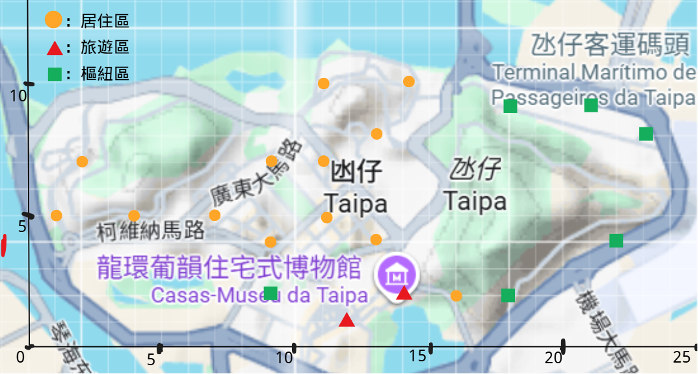
\includegraphics[width = \textwidth]{sections/images/投放.png}
    \caption{21處站點已標出的嘉模堂區地圖}
    \label{fig:cluster4_20}
\end{figure}
每個站點的初始投放量如下表所示.
\begin{table}[H]
    \begin{center}
        \begin{tabular}{ccccc}
        \hline
        站點編號 & 區域 & 對應坐標 & 實際地界 & 初始投放數量 \\
        \hline
        1 & 居住區 & (1,5) & 氹仔海洋花園衛生中心入口 & 5 \\
        2 & 居住區 & (2,7) & 海洋廣場入口 & 12 \\
        3 & 居住區 & (4,5) & 盈翠山莊馬路對面 & 8 \\
        4 & 居住區 & (7,5) & 澳門賽馬會賽事大樓入口左側 & 12 \\
        5 & 居住區 & (9,4) & 美景花園入口 & 15 \\
        6 & 居住區 & (9,7) & 鴻發花園入口右側 & 10 \\
        7 & 居住區 & (11,5) & 澳門大學附屬應用學校入口馬路對面 & 15 \\
        8 & 居住區 & (11,7) & 雄景花園入口 & 13 \\
        9 & 居住區 & (11,10) & 中福花園（麗怡閣）入口 & 10 \\
        10 & 居住區 & (13,4) & 泉悅花園入口 & 15 \\
        \vdots & \vdots & \vdots & \vdots & \vdots \\
        20 & 旅遊區 & (12,1) & 官也街 & 8 \\
        21 & 旅遊區 & (14,2) & 龍環葡韻 & 5 \\
        \hline
        \end{tabular}
    \end{center}
    \caption{共享單車站點的投放信息, {\color{red} \Large 附錄}}
\end{table}

\subsection{共享單車再平衡問題}
\subsubsection{目標函數}
為滿足用戶租還車需求, 運營商需要派遣調度卡車將共享單車從取貨點(初始庫存大於期望需求), 調送至送貨點(初始庫存小於期望需求), 以實現供求失衡站點的再平衡. 調度卡車從車場出發, 服務完一系列站點之後返回車場, 產生與之對應的運輸成本. 考慮到實際中卡車調度作業會受各種因素的限制(如預算限製與工作時長等), 為提高調度的靈活度, 本問題允許調度結果不滿足實際需求.即卡車可以在送貨點留下的單車數量小於期望需求, 或者在取貨點留下的單車數量大於期望需求. 然而若調度結果不滿足用戶需求, 會給用戶帶來不便, 因此我們需要一個與期望需求偏離時產生的懲罰成本\(p\).

本模型將該實際問題定義在有向圖\(G=(S_0, E)\)上. 其中站點集合\(S = P\cup D\)為取貨站點集合與卸貨站點集合的並集, \(S_0 = S\cup\{0\}\)為所有站點再額外加上車場\(0\). 邊集合\(E\)為所有站點之間的道路連接\(e\)(每條弧關聯運輸成本與運輸時間), 本問題需要確定卡車為哪些卡車提供服務、選擇哪些邊作為運輸路線以及在每一個站點的取貨與卸貨數量, 從而最小化總成本, 即為總運輸成本與懲罰成本之和.

該模型的目標函數為:
\begin{equation}
\min \sum_{i,j\in S_0}c_{ij}x_{ij} + \sum_{i\in S}\frac{p_i|s_i - s_i^I|}{s_i^I}
\end{equation}
其中\(c_{ij}\)為從站點\(i\)到站點\(j\)的運輸成本. 現實中\(c\)與路況、油耗以及員工薪水有關, 但為了簡化模型, 這裡認為\(c\)與運輸路程成正比例關係, 也就是認為\(c=k_c d(e_{ij})\), 其中\(d(e_{ij})\)為從站點\(i\)到站點\(j\)的道路長度.
\(x_{ij}\)為0-1變量, 表示是否選擇從站點\(i\)到站點\(j\)的邊.
\(p_i\)為站點\(i\)調度結束後庫存\(s_i(= s_i^0 - y_i)\)偏離期望需求\(s_i^I\)的懲罰成本. 
\subsubsection{庫存量約束}


調度貨車在每個站點的取貨數量\(y_i\)不能超過站點的初始庫存\(s_i^0\), 卸貨數量不能超過站點剩餘庫存\(l_i - s_i^0\),其中\(l_i\)為站點\(i\)的最大庫存. \(\sum_{j\in S_0}x_{ij}\)表示該站點是否被訪問, 如果被訪問則為1, 沒有被訪問則為0, 這樣就可以確保若該站點未被訪問, 則取貨數量與卸貨數量均為0.
\begin{gather}
y_i \leqslant s_i^0 \sum_{j\in S_0}x_{ij}, \forall i\in P\\
-y_i \leqslant \left(l_i - s_i^0\right)\sum_{j\in S_0}x_{ij}, \forall i\in D
\end{gather}
\subsubsection{流量約束}
根據{\color{red}\Large 假設}, 該模型不允許一輛卡車同時訪問一個站點多次, 因此對於每個站點\(i\), 其被訪問的邊\(x_{ij}\)的總和\(\sum x_{ij}\)需要小於等於1. 同時, 車場\(0\)需要被訪問一次, 而且卡車在最後必須回到車場, 於是得到以下兩個約束條件.
\begin{gather}
\sum_{j\in S_0}x_{ij} = \sum_{j\in S_0}x_{ji} \leqslant 1, \forall i\in S_0\\%每個站點只能被訪問一次
\sum_{j\in S_0}x_{0j} = \sum_{j\in S_0}x_{j0} = 1
\end{gather}
\subsubsection{貨車運載量約束}
接下來對貨車的運載量進行約束.若在出發時車場的庫存為\(g\), 則在出發時取貨量\(y_0\)以及貨車運載量\(Q_0\)為\(g\). 在每個站點進行裝貨以及卸貨操作後, 貨車的庫存量\(Q\)需要滿足以下約束條件. 若從站點\(i\)到站點\(j\)的邊被選擇, 則站點\(j\)的庫存量\(Q_j\)需要大於等於站點\(i\)的庫存量\(Q_i\)加上在i站點的取貨量(或卸貨量)\(y_i\). 當\(x_{ij} = 0\)時, 取一個充分大的常數\(M\), 即\(M(1-x_{ij})\)充分大, 使得\(Q_i + y_i -M(1-x_{ij})<0\), 令到該對\(Q\)的約束條件無效. 同時, 貨車在每個站點的運載量不能超過貨車的最大運載量\(C\). 相似地, 若該站點未被訪問, 則運載量為0.
\begin{gather}
Q_0 = y_0 =g \leqslant C\\
Q_j \geqslant Q_i + y_i - M(1-x_{ij}), \forall i,j\in S_0, i\neq j\\
Q_i \leqslant C\sum_{j\in S_0}x_{ij}, \forall i\in S_0
\end{gather}
\subsubsection{工作時間約束}
在運載過程中, 貨車的行駛時間不能超過預定的工作時間\(T_{工作}\). 記從站點\(i\)到站點\(j\)的行駛時間為\(t_{ij}\), 則在每個站點的行駛時間需要滿足以下約束條件. 規定從車場出發時的累計工作時間\(T_{累積}\) 為0. 在被訪問過的某個站點\(j\)上, 累計工作時間\({T_{累積}}_j \)需要大於等於從站點\(i\)到站點\(j\)的行駛時間\(t_{ij}\)加上在站點\(j\)的卸貨時間\(u_j\), 再加上在\(i\)點的累計工作時間\({T_{累積}}_i\). 而當\(j\)點未被訪問過時, 約束條件無效. 若貨車從\(i\)點返回車場, 則在\(i\)點的累計工作時間\({T_{累積}}_i \)加上從\(i\)點到車場的行駛時間\(t_{i0}\)需要小於等於預定的工作時間\(T_{工作}\).
\begin{gather}
{T_\text{累積}}_0 = 0\\
{T_\text{累積}}_j \geqslant {T_\text{累積}}_i + t_{ij} + u_j -  M(1-x_{ij}), \forall i\in S_0,j\in S, i\neq j\\
{T_\text{累積}}_i + t_{i0}(1-x_{i0}) \leqslant T,\forall i\in S
\end{gather}
在這裡, 根據{\color{red}\Large 假設}有每個站點的裝卸時間\(u_i \propto |y_i|\).

\subsubsection{多輛卡車調度模型}
該調度方案僅考慮了一台貨車的調度, 但實際中可能有多台貨車參與調度. 若該系統存在\(K\)輛調度卡車, 記為卡車集\(\mathcal{K}=\{1,2,\dots,K\}\). 每輛卡車有不同的運載量\(C^k\)與初始庫存\(g^k\), 並且每輛卡車的工作時間\(T^k\)也可能不同.在這種情況下, 我們需要對每輛卡車的調度進行建模. 對於每輛卡車\(k\), 我們可以定義一個與上述單輛卡車調度模型類似的目標函數:
\begin{equation}
\min \sum_{k\in \mathcal{K}}\sum_{i,j\in S_0}c_{ij}x_{ij}^k + \sum_{i\in S}p_i|s_i - s_i^{I}|
\end{equation}
其中\(x_{ij}^k\)表示卡車\(k\)是否選擇從站點\(i\)到站點\(j\)的邊, \(s_i^k\)為卡車\(k\)在站點\(i\)的庫存量, \(s_i^{I,k}\)為卡車\(k\)在站點\(i\)的期望需求. 
對於每輛卡車\(k\), 由於前文的所有約束條件均與卡車的整體調度方案無關, 因此我們可以將上述約束條件套用到每輛卡車上, 即為原有約束條件添加上標\(k\). 另外, 卡車\(k\)從倉庫出發時的庫存量\(g^k\)之和不能超過倉庫的總車輛, 但根據{\color{red}\Large 假設[]}, 倉庫有充分多的共享單車, 不會被卡車用盡. 

另外, 為了確保站點不會被不同卡車訪問多次, 我們需要對每個站點的訪問進行約束. 具體來說, 對於每個站點\(i\), 所有卡車\(k\)的訪問邊\(x_{ij}^k\)的總和需要小於等於1, 即
\begin{equation}
\sum_{k\in \mathcal{K}}\sum_{j\in S_0}x_{ij}^k \leqslant 1, \forall i\in S_0
\end{equation}

這樣就得到了多輛卡車調度模型的完整描述.

\subsubsection{模型參數的選取}
根據前文, 站點可以被分為樞紐區\(S_T\)、居民區\(S_R\)以及旅遊區\(S_H\), 即\(S = S_T\cup S_R\cup S_H\). 因此, 對於\(S\)中的每一個站點可以選擇不同的懲罰成本\(p_i\in\{p_T, p_R, p_H\}\). 具體來說, 樞紐區的懲罰成本\(p_T\)可以設置為0, 因為這些站點的期望需求通常較高且穩定,
而居民區的懲罰成本\(p_R\)可以設置為較低的值, 因為這些站點的期望需求較低且波動較大, 最後旅遊區的懲罰成本\(p_H\)可以設置為較高的值, 因為這些站點的期望需求通常較高且波動較大. 這樣的設置可以使得調度方案更符合實際需求, 並且能夠更好地平衡各個站點的庫存與需求. 若在其他城市中有其他適用的分區方案, 可以套用本模型進行參數的選取.

每段道路的運輸成本\(c_{ij}\)可以根據實際情況進行設置, 例如可以考慮道路的長度、交通狀況等因素. 對於每輛卡車的運載量\(C^k\)與初始庫存\(g^k\), 可以根據實際情況進行設置,例如可以考慮卡車的大小、載重能力等因素. 道路的長度\(d(e)\)可以通過市面上的導航係統獲取(如高德地圖、百度地圖等), 而道路的交通狀況可以通過實時交通數據獲取(如高德地圖的實時路況數據).
對於每個站點的裝卸時間\(u_i\), 可以根據實際情況進行設置, 例如可以考慮站點員工的工作效率. 同樣地,每位員工的工作時間\(T_\text{工作}^k\)也可以根據實際情況進行設置. 這些參數的選取可以根據實際情況進行調整, 以使得調度方案更符合實際需求.

\subsubsection{模型求解與調度信息}
考慮到在實際中搜集\(N\)個站點兩兩之間的距離將產生\(N(N-1)\)條有向邊, 因此該模型的計算量較大. 因此, 在此模型中, 我們將使用兩點之間的曼哈頓距離, 即對於點\(\mathbf{x}\)和\(\mathbf{y}\), 其曼哈頓距離為
\begin{equation}
d(\mathbf{x}, \mathbf{y}) = |x_1 - y_1| + |x_2 - y_2|
\end{equation}
這樣可以大大減少計算量, 並且在實際中也能夠較好地反映兩點之間的距離.
另外, 由於用戶的騎車行為難以預測, 並且在澳門未有足夠的歷史數據進行訓練, 因此我們將利用幾組隨機數作為原投放量, 將前文的初始投放數量作為目標投放量進行優化.
對於其他的參數, 我們將根據前文的討論進行設置. 
\begin{enumerate}
    \item 最大庫存設置為\(l_i=\left\lceil 150\% s_i^I  \right\rceil\).
    為了確保每個站點歸還單車時有樁可用, 我們將站點的最大庫存設置為期望需求的150\%, 這樣可以確保在還車時有充分的餘量.
    \item 根据《道路旅客運輸企業安全管理規範》相關要求, 貨車的最大工作時間\(T_\text{工作}= 120 \text{min}\).
    \item 貨車的最大運載量\(C= 40\), 這是根據澳門的道路狀況以及貨車的實際情況進行設置的. 澳門道路狹窄, 貨車的運載量需要控制在一定範圍內, 以確保道路安全.
    \item 根據不同地區(居住區、旅遊區、樞紐區)的需求特點, 我們將懲罰成本設置為
    \begin{itemize}
        \item 居民區\(p_T=200\), 因為這些站點的期望需求通常較高且穩定, 不需要懲罰成本;
        \item 樞紐區\(p_R=400\), 因為這些站點的期望需求較低且波動較大, 需要一定的懲罰成本來平衡庫存與需求;
        \item 旅遊區\(p_H=600\), 因為這些站點的期望需求通常較高且波動較大, 需要較高的懲罰成本來平衡庫存與需求.
    \end{itemize}
    並且, 通過數值試驗, 該參數與距離的數量級相當, 這樣可以確保懲罰成本在目標函數中有足夠的影響力.
    \item 裝卸時間係數設置為\(k_u = 0.2 \text{min/車}\). 這是根據實際情況決定的.
    \item 運輸成本設置為\(c_{ij} = d(e_{ij})\). 
    \item 根據{\color{red} \Large 假設}, 車輛到達下一個站點的時間正比於站點之間的距離, 即\(t_{ij} = k_td(e_{ij})\). 在這裡將\(k_t\)設置為\(0.00167\text{min/km}\), 約每小時40公里的速度.
\end{enumerate}
將參數輸入到{\color{red}\Large 附錄}的程序中, 測試用例(即每個站點的自行車數量)如{\color{red} \Large 附錄[]所示}, 運行得到以下結果. 
\begin{table}[H]
    \begin{center}
        \begin{tabular}{cccccccccc}
            \hline
            站点  & 区域 & 操作量 & 初始库存 & 最终库存 & 期望库存 & 库存偏差 & 是否访问 & 惩罚成本 \\
            \hline
            4  & 居住區 & 4.0 & 16 & 12.0 & 12 & 0.0 & 是 & 0.0 \\
            5  & 居住區 & 5.0 & 20 & 15.0 & 15 & 0.0 & 是 & 0.0 \\
            14  & 樞紐區 & 1.0 & 26 & 25.0 & 25 & 0.0 & 是 & 0.0 \\
            19  & 樞紐區 & -20.0 & 10 & 30.0 & 30 & 0.0 & 是 & 0.0 \\
            2  & 居住區 & -12.0 & 0 & 12.0 & 12 & 0.0 & 是 & 0.0 \\
            18  & 樞紐區 & -5.0 & 20 & 25.0 & 25 & 0.0 & 是 & 0.0 \\
            9  & 居住區 & 0.0 & 9 & 9.0 & 10 & 1.0 & 否 & 1000.0 \\
            11  & 居住區 & 0.0 & 5 & 5.0 & 8 & 3.0 & 否 & 3000.0 \\
            12  & 居住區 & 0.0 & 3 & 3.0 & 10 & 7.0 & 否 & 7000.0 \\
            15  & 樞紐區 & 0.0 & 13 & 13.0 & 14 & 1.0 & 否 & 2000.0 \\
            21  & 旅遊區 & 0.0 & 7 & 7.0 & 5 & 2.0 & 否 & 6000.0 \\
            \hline
        \end{tabular}
    \end{center}
    \caption{調度完成後的站點信息}
\end{table}
\begin{table}[H]
    \begin{center}
        \begin{tabular}{cccccc}
            \hline
            从站点 & 到站点 & 距离(米) & 操作量 & 操作时间 & 累计时间(分) \\
            \hline
            0 & 14 & 4200.0 & 0.0 & 0.00 & 7.01 \\
            14 & 5 & 900.0 & 1.0 & 0.20 & 8.71 \\
            5 & 4 & 450.0 & 5.0 & 1.00 & 10.46 \\
            4 & 13 & 2250.0 & 4.0 & 0.80 & 14.61 \\
            13 & 19 & 1200.0 & 0.0 & 0.00 & 16.61 \\
            19 & 18 & 1200.0 & -20.0 & 4.00 & 22.61 \\
            18 & 2 & 31500.0 & -5.0 & 1.00 & 76.11 \\
            2 & 0 & 34500.0 & -12.0 & 2.40 & 115.51 \\
            \hline
        \end{tabular}
    \end{center}
    \caption{貨車調度路線以及在該站點的裝卸信息}
\end{table}

在該調度方式下, 總成本為34000(無量綱), 其中運輸成本為15500, 懲罰成本為19000.

在這裡由於約束條件較緊, 卡車無法再固定的容量和時間內滿足所有站點的需求, 例如站點9的期望需求為\(s_i^I=10\), 但調度結果為\(s_i=9\)(未訪問), 即該站點的庫存量小於期望需求, 
因此產生了懲罰成本. 但這已經是在該約束條件下令目標函數最小化的結果, 若需要滿足這些站點的全部需求, 我們需要放寬約束條件或者調度另一輛卡車同時進行共享單車的調度作業.